% Method of Moments

\frame{ \frametitle{Method of Moments: Overview}
  Now we're going to derive the approximation!
  \pause

  Game plan:
  \pause
  \begin{enumerate}
    \uncover<+->{\item Find the first three moments about the mean (central moments) of the binomial and the skew-normal.\\}
          \uncover<+->{\vspace{2mm}
                       What are central moments?: $E(X)$, $E([X - E(X)]^2)$, $E([X - E(X)]^3)$.}
    \uncover<+->{\item Set them equal to each other.}
    \uncover<+->{\item Take $n$ and $p$ to be constants; solve for $\mu$, $\sigma$, and $\lambda$.}
  \end{enumerate}
}

%% The Central Moments of the Binomial
\frame{ \frametitle{Method of Moments: Central Moments of the Binomial}
  Let's start with the binomial ...
}
\frame{ \frametitle{Method of Moments: Central Moments of the Binomial}
  Let $B \sim Bin(n,p)$.
  \pause

  The first two central moments of $B$ are just the mean and variance:
  \pause
  \begin{align*}
    E(B) &= np \\
    E([B - E(B)]^2) &= Var(B) = np(1-p)
  \end{align*}
}
\frame{ \frametitle{Method of Moments: Central Moments of the Binomial}
  The third one takes some elbow grease.
  \pause

  First we'll need to find $E(B^2)$ and $E(B^3)$.
}
\frame{ \frametitle{Method of Moments: Central Moments of the Binomial}
  Recall that $Var(B) = E(B^2) - [E(B)]^2$. \pause Thus
  \begin{align*}
    \uncover<+->{E(B^2) &= Var(B) + [E(B)]^2 \\}
    \uncover<+->{&= np(1-p) + n^2p^2 \\}
    \uncover<+->{&= np - np^2 + n^2p^2.}
  \end{align*}
}
\frame{ \frametitle{Method of Moments: Central Moments of the Binomial}
  We will get $E(B^3)$ via the third factorial moment, E[B(B-1)(B-2)].
}
\frame{ \frametitle{Method of Moments: Central Moments of the Binomial}
  \begin{align*}
    \uncover<+->{&E[B(B-1)(B-2)] \\}
    \uncover<+->{&= \sum_{x=0}^n x (x-1) (x-2) \cdot \left\{ \binom{n}{x} p^x q^{n-x} \right\} \\}
    \uncover<+->{&= \sum_{x=3}^n x (x-1) (x-2) \cdot \left\{ \binom{n}{x} p^x q^{n-x} \right\} \\}
    \uncover<+->{&= \sum_{x=3}^n x(x-1)(x-2) \cdot \frac{n!}{x!\;(n-x)!} \; p^x q^{n-x} \\}
    \uncover<+->{&= \sum_{x=3}^n \frac{n!}{(x-3)!\;(n-x)!} \; p^x q^{n-x} \\}
    \uncover<+->{&= \sum_{x=3}^n n(n-1)(n-2) p^3 \cdot \frac{(n-3)!}{(x-3)!\;(n-x)!} \; p^{x-3}q^{n-x} \\}
  \end{align*}
}
\frame{ \frametitle{Method of Moments: Central Moments of the Binomial}
  \begin{align*}
    \uncover<+->{&= \sum_{x=3}^n n(n-1)(n-2) p^3 \cdot \frac{(n-3)!}{(x-3)!\;(n-x)!} \; p^{x-3}q^{n-x}}
    \uncover<+->{\intertext{Let $y=x-3$; then $x=y+3$, and $x=3$, $x=n \Ra y=0$, $y=n-3$:}}
    \uncover<+->{&= n(n-1)(n-2)p^3 \cdot \sum_{y=0}^{n-3} \frac{(n-3)!}{y!\;(n-(y+3))!} \; p^y q^{n-(y+3)} \\}
    \uncover<+->{&= n(n-1)(n-2)p^3 \cdot \underbrace {\sum_{y=0}^{n-3} \frac{(n-3)!}{y!\;((n-3)-y)!} \; p^y q^{(n-3)-y}}_{\mathclap{\textnormal{[pdf of $Bin(n-3,p)$ summed over its domain] = 1}}} \\}
    \uncover<+->{&= n(n-1)(n-2)p^3 \\}
    \uncover<+->{&= n^3p^3 - 3n^2p^3 + 2np^3}
  \end{align*}
}
\frame{ \frametitle{Method of Moments: Central Moments of the Binomial}
  To get $E(B^3)$, we expand the left side of the previous equation:
  \pause
  \begin{align*}
    \uncover<+->{&E[B(B-1)(B-2)] \\}
    \uncover<+->{&= E \left[ B^3 - 3B^2 + 2B \right] \\}
    \uncover<+->{&= E(B^3) - 3E(B^2) + 2E(B) \\}
    \uncover<+->{&= E(B^3) - 3(np - np^2 + n^2p^2) + 2np \\}
    \uncover<+->{&= E(B^3) - 3np + 3np^2 - 3n^2p^2 + 2np \\}
    \uncover<+->{&= E(B^3) + 3np^2 - 3n^2p^2 - np}
  \end{align*}
}
\frame{ \frametitle{Method of Moments: Central Moments of the Binomial}
  Left side: $E(B^3) + 3np^2 - 3n^2p^2 - np$

  Right side: $n^3p^3 - 3n^2p^3 + 2np^3$
  \pause

  Set them equal and solve for $E(B^3)$:
  \pause
  \begin{align*}
    \uncover<+->{&E(B^3) + 3np^2 - 3n^2p^2 - np = n^3p^3 - 3n^2p^3 + 2np^3 \\}
    \uncover<+->{&\Rightarrow \qquad E(B^3) = n^3p^3 - 3n^2p^3 + 2np^3 - 3np^2 + 3n^2p^2 + np}
  \end{align*}
}
\frame{ \frametitle{Method of Moments: Central Moments of the Binomial}
  Now we can (finally!) compute the third central moment:
  \pause
  \begin{align*}
    \uncover<+->{&E \left( [B - E(B)]^3 \right) \\}
    \uncover<+->{&= E \left( B^3 - 3B^2 E(B) + 3B [E(B)]^2 - [E(B)]^3 \right) \\}
    \uncover<+->{&= E(B^3) - 3 E(B^2) E(B) + 3 E(B) [E(B)]^2 - [E(B)]^3 \\}
    \uncover<+->{&= E(B^3) - 3 E(B^2) E(B) + 2 [E(B)]^3 \\}
    \uncover<+->{&= (n^3p^3 - 3n^2p^3 + 2np^3 - 3np^2 + 3n^2p^2 + np) \\
                 &\quad - 3(np - np^2 + n^2p^2)(np) + 2(np)^3 \\}
    \uncover<+->{&= \cancel{n^3p^3} - \cancel{3n^2p^3} + 2np^3 - 3np^2 + \cancel{3n^2p^2} + np \\
                 &\quad - \cancel{3n^2p^2} + \cancel{3n^2p^3} - \cancel{3n^3p^3} + \cancel{2n^3p^3} \\}
    \uncover<+->{&= 2np^3 - 3np^2 + np \\}
    \uncover<+->{&= np(p-1)(2p-1)}
  \end{align*}
}
\frame{ \frametitle{Method of Moments: Central Moments of the Binomial}
  Let's restate our results:
  \begin{align*}
    E(B) &= np, \\
    E([B - E(B)]^2) &= np(1-p), \\
    E([B - E(B)]^3) &= np(p-1)(2p-1)
  \end{align*}
}

%% The Central Moments of the Skew-Normal
\frame{ \frametitle{Method of Moments: Central Moments of the Skew-Normal}
  Now lets move on to skew-normal ...
}
\frame{ \frametitle{Method of Moments: Central Moments of the Skew-Normal}
  Let $Y \sim SN(\mu, \sigma, \lambda)$.
  \pause

  Again, the first and second central moments of $Y$ are the mean and variance.
  \pause
  \begin{align*}
    E(Y) &= \mu + b \delta \sigma \\
    Var(Y) &= \sigma^2 (1 - b^2 \delta^2)
  \end{align*}
}
\frame{ \frametitle{Method of Moments: Central Moments of the Skew-Normal}
  Again, the third one is a little harder:
  \pause
  \begin{align*}
    \uncover<+->{&E([Y - E(Y)]^3) \\}
    \uncover<+->{&= E(Y^3) - 3E(Y^2)E(Y) + 2[E(Y)]^3 \\}
    \uncover<+->{&= (\mu^3 + 3 b \delta \mu^2 \sigma + 3 \mu \sigma^2 + 3 b \delta \sigma^3 - b \delta^3 \sigma^3) \\
                 &\quad - 3 (\mu^2 + 2b \delta \mu \sigma + \sigma^2) (\mu + b \delta \sigma) + 2\;(\mu + b \delta \sigma)^3 \\}
    \uncover<+->{&= \cancel{\mu^3} + \cancel{3 b \delta \mu^2 \sigma} + \cancel{3 \mu \sigma^2} + \cancel{3 b \delta \sigma^3} - b \delta^3 \sigma^3 - \cancel{3 \mu^3} - \cancel{3 b \delta \mu^2 \sigma} \\
                 &\quad - \cancel{6 b \delta \mu^2 \sigma} - \cancel{6 b^2 \delta^2 \mu \sigma^2} - \cancel{3 \mu \sigma^2} - \cancel{3 b \delta \sigma^3} + \cancel{2 \mu^3} + \cancel{6 b \delta \mu^2 \sigma} \\
                 &\quad + \cancel{6 b^2 \delta^2 \mu \sigma^2} + 2 b^3 \delta^3 \sigma^3 \\}
    \uncover<+->{&= 2 b^3 \delta^3 \sigma^3 - b \delta^3 \sigma^3 \\}
    \uncover<+->{&= b \delta^3 \sigma^3 (2b^2 - 1)}
  \end{align*}
}
\frame{ \frametitle{Method of Moments: Central Moments of the Skew-Normal}
  Our results, restated:
  \begin{alignat*}{4}
    E(Y) &= \mu + b \delta \sigma \;&=&\; \mu + \sigma \cdot \sqrt{\frac{2}{\pi}} \cdot \frac{\lambda}{\sqrt{1 + \lambda^2}} \\
    E([Y - E(Y)]^2) &= \sigma^2 (1 - b^2 \delta^2) \;&=&\; \sigma^2 \left( 1 - \frac{2}{\pi} \cdot \frac{\lambda^2}{1 + \lambda^2} \right) \\
    E([Y - E(Y)]^3) &= b \delta^3 \sigma^3 (2b^2 - 1) \;&=&\; \sigma^3 \sqrt{\frac{2}{\pi}} \left( \frac{\lambda}{\sqrt{1 + \lambda^2}} \right)^3 \left( \frac{4}{\pi} - 1 \right)
  \end{alignat*}
}

%% Deriving an Approximation
\frame{ \frametitle{Method of Moments: Deriving an Approximation}
  We're finally ready to derive our approximation!
}
\frame{ \frametitle{Method of Moments: Deriving an Approximation}
  We start by setting the central moments of the binomial equal to the central moments of the skew-normal.
  \pause
  \begin{subequations}
    \begin{align}
      \uncover<+->{np &= \mu + \sigma \cdot \sqrt{\frac{2}{\pi}} \cdot \frac{\lambda}{\sqrt{1 + \lambda^2}} \label{eq:first-moment-set} \\}
      \uncover<+->{np(1-p) &= \sigma^2 \left( 1 - \frac{2}{\pi} \cdot \frac{\lambda^2}{1 + \lambda^2} \right) \label{eq:second-moment-set} \\}
      \uncover<+->{np(p-1)(2p-1) &= \sigma^3 \sqrt{\frac{2}{\pi}} \left( \frac{\lambda}{\sqrt{1 + \lambda^2}} \right)^3 \left( \frac{4}{\pi} - 1 \right) \label{eq:third-moment-set} \\}
      \notag
    \end{align}
  \end{subequations}
}
\frame{ \frametitle{Method of Moments: Deriving an Approximation}
  To get $\lambda$, divide the cube of \eqref{eq:second-moment-set} by the
  square of \eqref{eq:third-moment-set}:
  \pause
  \begin{align}
    \uncover<+->{\frac{\sigma^6 \left( 1 - \frac{2}{\pi} \cdot \frac{\lambda^2}{1 + \lambda^2} \right)^3}{\sigma^6 \cdot \frac{2}{\pi} \left( \frac{\lambda}{\sqrt{1 + \lambda^2}} \right)^6 \left(
                 \frac{4}{\pi} - 1 \right)^2} &= \frac{n^3p^3(1-p)^3}{n^2p^2(p-1)^2(2p-1)^2} \nonumber \\}
    \uncover<+->{\Rightarrow \quad \frac{\left( 1 - \frac{2}{\pi} \cdot \frac{\lambda^2}{1+\lambda^2} \right)^3}{\frac{2}{\pi} \left( \frac{\lambda^2}{1+\lambda^2} \right)^3 \left( \frac{4}{\pi} - 1
                 \right)^2} &= \frac{np(1-p)}{(1-2p)^2} \label{eq:solving-for-lambda} \\}
    \notag
  \end{align}
}
\frame{ \frametitle{Method of Moments: Deriving an Approximation}
  Equation \eqref{eq:solving-for-lambda} can be solved for $\lambda^2$.
  \pause

  Then take $\lambda$ to be
  \begin{equation*}
    \lambda = \textnormal{\{sign of $(1-2p)$\}} \sqrt{\lambda^2}.
  \end{equation*}
  \pause

  Why?
  \pause
  Recall Property 3 ...
}
\frame{ \frametitle{Method of Moments: Deriving an Approximation}
  \begin{center}
    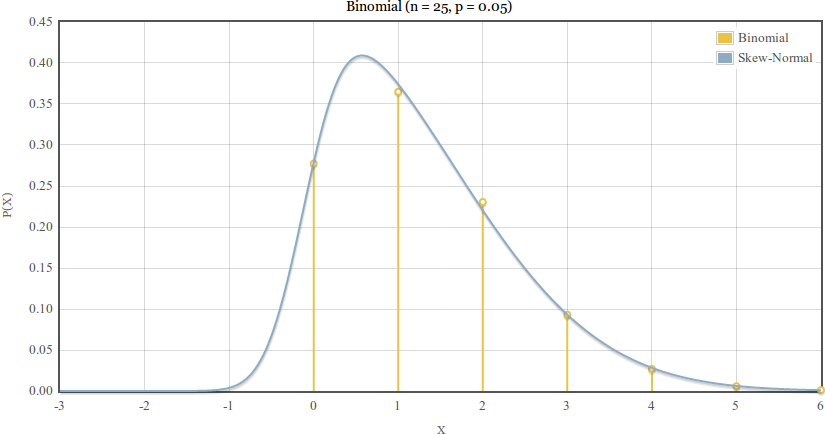
\includegraphics[width=\textwidth]{../images/binomial-sn-n25p005.png}
  \end{center}
  When $p < 0.5$:
  \pause
  \begin{itemize}[<+->]
    \item The binomial skews right (weight shifts left) and approaches $+|N(0,1)|$ $\lra$ $\lambda$ is positive
    \item $(1-2p)$ is positive
  \end{itemize}
}
\frame{ \frametitle{Method of Moments: Deriving an Approximation}
  \begin{center}
    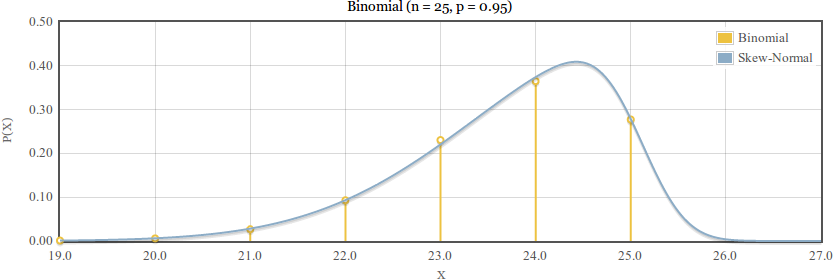
\includegraphics[width=\textwidth]{../images/binomial-sn-n25p095.png}
  \end{center}
  When $p > 0.5$:
  \pause
  \begin{itemize}[<+->]
    \item The binomial skews left (weight shifts right) and approaches $-|N(0,1)|$ $\lra$ $\lambda$ is negative
    \item $(1-2p)$ is negative
  \end{itemize}
}
\frame{ \frametitle{Method of Moments: Deriving an Approximation}
  Once you have $\lambda$, solve for $\sigma$ and then $\mu$.
  \pause
  \begin{equation*}
    \uncover<+->{np(1-p) = \sigma^2 \left( 1 - \frac{2}{\pi} \cdot \frac{\lambda^2}{1 + \lambda^2} \right) \quad\Rightarrow\quad
                 \sigma = \sqrt{\frac{np(1-p)}{1 - \frac{2}{\pi} \cdot \frac{\lambda^2}{1 + \lambda^2}}}}
  \end{equation*}
  \begin{equation*}
    \uncover<+->{np = \mu + \sigma \cdot \sqrt{\frac{2}{\pi}} \cdot \frac{\lambda}{\sqrt{1 + \lambda^2}} \quad\Rightarrow\quad
                 \mu = np - \sigma \cdot \sqrt{\frac{2}{\pi}} \cdot \frac{\lambda}{\sqrt{1 + \lambda^2}}}
  \end{equation*}
}
\frame{ \frametitle{Method of Moments: Deriving an Approximation}
  When $p = 0.5$, the right hand side of \eqref{eq:solving-for-lambda}
  \begin{equation*}
    \frac{\left( 1 - \frac{2}{\pi} \cdot \frac{\lambda^2}{1+\lambda^2} \right)^3}{\frac{2}{\pi} \left( \frac{\lambda^2}{1+\lambda^2} \right)^3 \left( \frac{4}{\pi} - 1 \right)^2}
    = \frac{np(1-p)}{(1-2p)^2}
  \end{equation*}
  is undefined.
  \pause

  Uh-oh.
}
\frame{ \frametitle{Method of Moments: Deriving an Approximation}
  Fortunately, our intuition rescues us:
  \pause

  When $p=0.5$, the binomial is symmetric, so $\lambda$ should equal 0.
  \pause

  This takes us back to the usual normal approximation:
  \pause
  \begin{align*}
    \uncover<+->{\sigma &= \sqrt{\frac{np(1-p)}{1 - \frac{2}{\pi} \cdot \frac{0^2}{1 + 0^2}}} = \sqrt{\frac{np(1-p)}{1}} = \sqrt{np(1-p)} \\}
    \uncover<+->{\mu &= np - \sigma \cdot \sqrt{\frac{2}{\pi}} \cdot \frac{0}{\sqrt{1 + 0^2}}  = np - 0 = np}
  \end{align*}
}

%% Restrictions
\frame{ \frametitle{Method of Moments: Restrictions}
  Unfortunately, though better than the normal approximation, our skew-normal method isn't universal.
}
\frame{ \frametitle{Method of Moments: Restrictions}
  To be able to solve for $\lambda$, we must restrict $n$ and $p$ by the following equation:
  \pause
  \begin{equation}
    np(1-p) \geq (1-2p)^2 \label{eq:solving-the-restriction}
  \end{equation}
  \pause
  From \eqref{eq:solving-the-restriction}, we can answer two questions:
}
\frame{ \frametitle{Method of Moments: Restrictions}
  \vspace{5mm}
  One: Given $p$, what is the least $n$ necessary?
  \pause
  \begin{equation*}
    n \geq \frac{(1-2p)^2}{p(1-p)}
  \end{equation*}
  \pause
  \begin{center}
    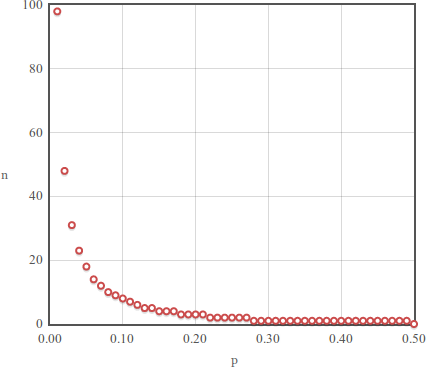
\includegraphics[width=0.7\textwidth]{../images/restriction-least-n.png}
  \end{center}
}
\frame{ \frametitle{Method of Moments: Restrictions}
  \vspace{5mm}
  Two: Given $n$, what is the range of possible $p$'s?
  \pause
  \begin{equation*}
    \frac12 - \frac12 \sqrt{\frac{n}{n+4}} \; \leq \; p \; \leq \; \frac12 + \frac12 \sqrt{\frac{n}{n+4}}
  \end{equation*}
  \pause
  \begin{center}
    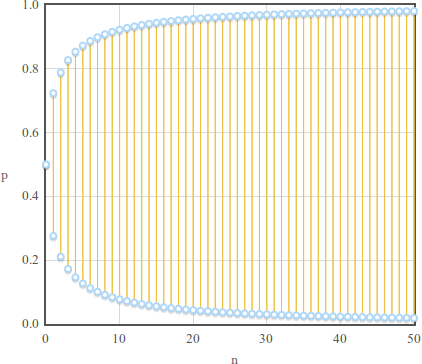
\includegraphics[width=0.7\textwidth]{../images/restriction-p-range.png}
  \end{center}
}
